\end{document}
$Header$

\documentclass{beamer}

% This file is a solution template for:

% - Talk at a conference/colloquium.
% - Talk length is about 20min.
% - Style is ornate.



% Copyright 2004 by Till Tantau <tantau@users.sourceforge.net>.
%
% In principle, this file can be redistributed and/or modified under
% the terms of the GNU Public License, version 2.
%
% However, this file is supposed to be a template to be modified
% for your own needs. For this reason, if you use this file as a
% template and not specifically distribute it as part of a another
% package/program, I grant the extra permission to freely copy and
% modify this file as you see fit and even to delete this copyright
% notice. 


\mode<presentation>
{
  % \usetheme{Warsaw}
  \usetheme{Madrid}
  % or ...

  % \setbeamercovered{transparent}
  \setbeamercovered{invisible}
  % or whatever (possibly just delete it)
}


\usepackage[english, russian]{babel}
% or whatever

\usepackage[utf8]{inputenc}
% or whatever

\usepackage{times}
\usepackage[T2A]{fontenc}

\usepackage{icomma}

\usepackage{tikz}
\usetikzlibrary{arrows}
\usepackage{expdlist}
\usepackage{cmap}
\usepackage{array}
\usepackage{xspace}
\usepackage{wrapfig}
\usepackage{srcltx}
\usepackage{epsfig}
\usepackage{verbatim}
\usepackage{listings}
\usepackage{placeins}
\usepackage{caption}
\usepackage{subfigure}
\usepackage{easytable}
\usepackage{fancybox}
\usepackage{multirow}

\captionsetup{labelformat=empty,labelsep=none}
% Or whatever. Note that the encoding and the font should match. If T1
% does not look nice, try deleting the line with the fontenc.


\title[Augmentation]{Augmentation}

\author[А. Латышев]{Алексей Латышев, группа M4139}

\institute[Университет ИТМО]
{
  кафедра Компьютерных технологий\\
  факультет Информационных Технологий и Программирования\\
  Университет ИТМО  
}
% - Use the \inst command only if there are several affiliations.
% - Keep it simple, no one is interested in your street address.

\date[ML 2018]{27 июня 2018}
%\date[CFP 2003] % (optional, should be abbreviation of conference name)
%{Conference on Fabulous Presentations, 2003}
% - Either use conference name or its abbreviation.
% - Not really informative to the audience, more for people (including
%   yourself) who are reading the slides online

% \subject{Theoretical Computer Science}
% This is only inserted into the PDF information catalog. Can be left
% out. 



% If you have a file called "university-logo-filename.xxx", where xxx
% is a graphic format that can be processed by latex or pdflatex,
% resp., then you can add a logo as follows:

% \pgfdeclareimage[height=0.5cm]{university-logo}{itmo_logo_rus_vert_blue.eps}
% \pgfdeclareimage[height=1.5cm]{university-logo}{itmo_small_white_rus.png}
\pgfdeclareimage[height=1cm]{university-logo}{itmo_horiz_white_rus.png}
\logo{\pgfuseimage{university-logo}}



% % Delete this, if you do not want the table of contents to pop up at
% % the beginning of each subsection:
% \AtBeginSection[]
% {
% \begin{frame}<beamer>{Содержание}
% \tableofcontents[currentsection]
%   \end{frame}
% }

%\AtBeginSubsection[]
%{
%  \begin{frame}<beamer>{Outline}
%    \tableofcontents[currentsection, currentsubsection]
%  \end{frame}
%}


% If you wish to uncover everything in a step-wise fashion, uncomment
% the following command: 

%\beamerdefaultoverlayspecification{<+->}

\makeatletter
\let\@@magyar@captionfix\relax
\makeatother
\begin{document}

\begin{frame}
  \titlepage
\end{frame}

%\begin{frame}{Outline}
%  \tableofcontents
  % You might wish to add the option [pausesections]
%\end{frame}


% Structuring a talk is a difficult task and the following structure
% may not be suitable. Here are some rules that apply for this
% solution: 

% - Exactly two or three sections (other than the summary).
% - At *most* three subsections per section.
% - Talk about 30s to 2min per frame. So there should be between about
%   15 and 30 frames, all told.

% - A conference audience is likely to know very little of what you
%   are going to talk about. So *simplify*!
% - In a 20min talk, getting the main ideas across is hard
%   enough. Leave out details, even if it means being less precise than
%   you think necessary.
% - If you omit details that are vital to the proof/implementation,
% just say so once. Everybody will be happy with that.

\begin{frame}
  \frametitle{Что это? И зачем?}
  Augmentation~--- с английского увеличение, прирост. В рамках машинного
  обучения термин означает <<раздувание>> датасета для достижения одной из двух
  целей:
  \pause
  \begin{itemize}[<+->]
  \item Увеличить тренировочную выборку в случае, когда данных очень мало.
    Например, это используется в медицине в распознавании по картинки
    какой-нибудь сложной опухоли. Здесь фотографий распознавемого объекта очень
    мало, приходится как-то решать эту проблему.
  \item Увеличить <<разнообразность>> представленных в тренировочном датасете
    картинок. В основном, как средство борьбы с переобучением. В работе
    исследовалась именно эта составляющая.
  \end{itemize}
  \pause
  Далее мы будем рассматривать только задачи, входными данными которых являются
  картинки. 
\end{frame}


\begin{frame}
  \frametitle{Как?}
  Один из способов это делать~--- различные <<геометрические>> преобразования над
  картинкой:
  \begin{enumerate}[<+->]
  \item Различные аффинные преобразования
    \begin{itemize}
    \item Повороты
    \item Отражения
    \item Сжатия к прямой
    \item Масштабирование
    \end{itemize}
  \item Различные проективные преобразования
    \begin{itemize}
    \item Наклоны
    \end{itemize}
  \item Обрезка    
  \end{enumerate}
\end{frame}

\begin{frame}
  \frametitle{Как? Random erasing.}
  \minipage{0.6\textwidth}
  Еще один пример Augmentation. С каждой картинкой перед тем как скормить ее на
  обучение модели с вероятностью $p$ сделают следующее. Выберут рандомный
  прямоугольник на картинке и заменят его на белый шум, либо закрасят серым
  цветом. Подробнее можно посмотреть в статье
  \href{https://arxiv.org/pdf/1708.04896.pdf}
  {https://arxiv.org/pdf/1708.04896.pdf}
  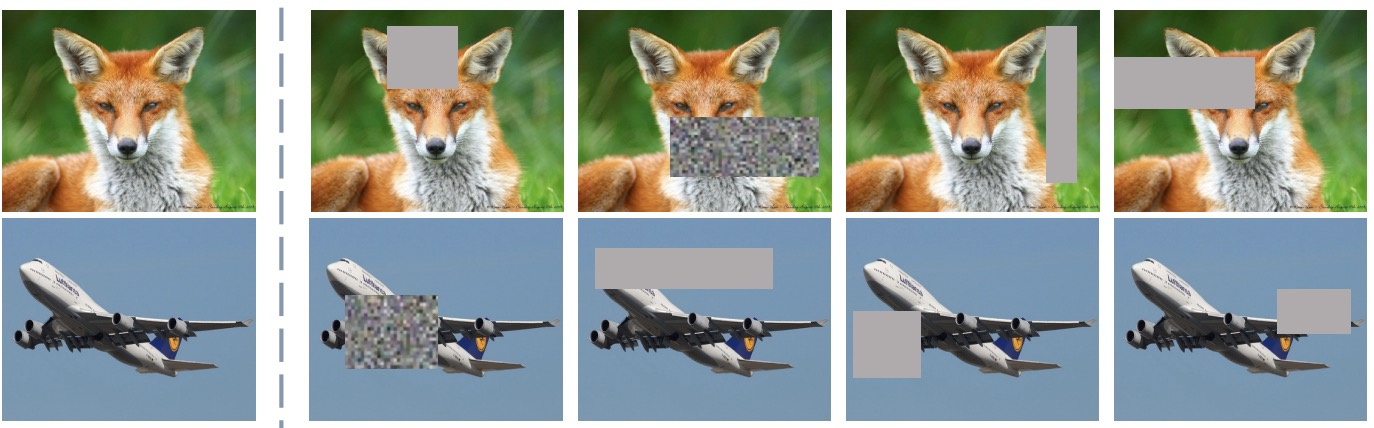
\includegraphics[width=1\textwidth]{erasing.jpg}
  \endminipage
  \minipage{0.4\textwidth}
  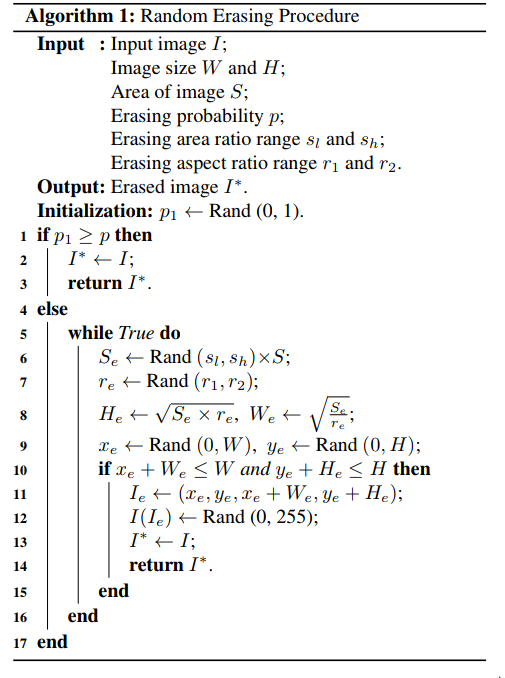
\includegraphics[width=1\textwidth]{random_erasing_algo.png}
  \endminipage
\end{frame}

\begin{frame}
  \frametitle{Как? Dropout.}
  Это не совсем Augmentation, но рядом. Dropout~--- рандомное выключение
  некоторых вершин в слое нейронной сети. А точнее каждая вершина слоя, к
  которой применен dropout с вероятностью $p$ даст нулевой вклад в следующий
  слой, на данном этапе обучения. При этом во время теста все вершины уже
  включены. Подробнее 
  \href{https://www.cs.toronto.edu/~hinton/absps/JMLRdropout.pdf}
  {https://www.cs.toronto.edu/~hinton/absps/JMLRdropout.pdf}
  \begin{center}
  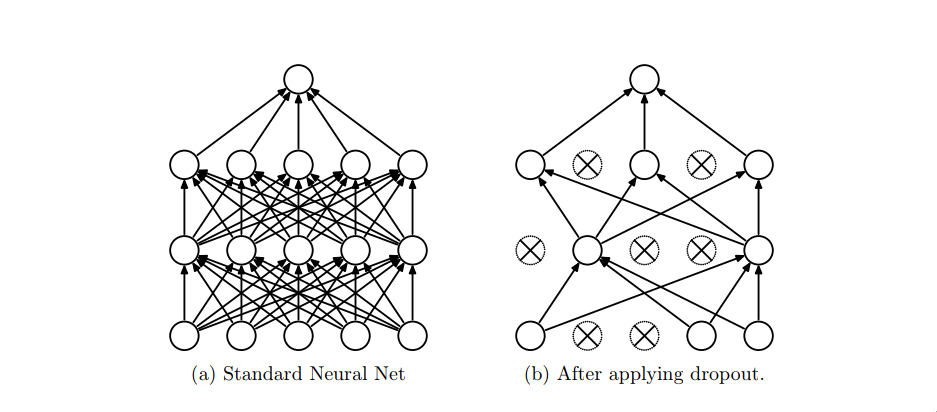
\includegraphics[trim=0 0 0 1cm, width=0.7\textwidth]{dropout.png}
  \end{center}
\end{frame}

\begin{frame}
  \frametitle{Как? Больше нейронных сетей \dots}
  Еще Augmentation можно делать с помощью нейронных сетей и обучать вместе с
  моделью. Получается неплохо.
  \begin{enumerate}
  \item GAN
  \item AugNet предложенный в
    \href{http://cs231n.stanford.edu/reports/2017/pdfs/300.pdf}
    {http://cs231n.stanford.edu/reports/2017/pdfs/300.pdf}
    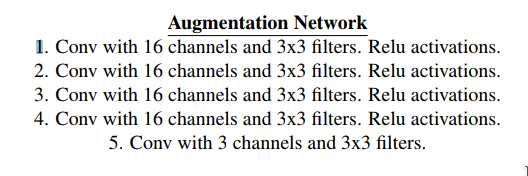
\includegraphics[width=0.5\textwidth]{augnet.png}
  \end{enumerate}
\end{frame}

\begin{frame}
  \frametitle{Что я делал?}
  Основная цель проверить, как влияет Augmentation на точность обучения.
  Для этого рассмотрим несколько датасетов и несколько архитектур нейронных
  сетей. Обучим, применяя и не применяя различные методы Augmentation. Сравним
  точность и итоговый средний loss. 
\end{frame}

\begin{frame}
  \frametitle{Датасеты и особенности обучения}
  \begin{enumerate}
  \item MNIST
  \item FashionMNIST
  \item CIFAR10
  \end{enumerate}
  
\end{frame}

\begin{frame}
  \frametitle{Результаты}
  \small
  \begin{tabular}[H]{|m{1.2cm}|m{2cm}|c|c|c|}
    \hline
    \multicolumn{2}{|c|}{Augmentation} & Simple         & Conv             & LeNet \\
    \hline
    \multirow{2}{*}{MNIST} & without & 0.1140 | 96.80\% & 0.0490 | 98.39\% & ?     \\
    \cline{2-5}
                           & ROT(10) & 0.1086 | 96.89\% & 0.0498 | 98.46\% & ?     \\

    \hline
    \multirow{2}{*}{Fashion} & without & 0.3874 | 86.40\% & 0.4030 | 84.95\% & ?\\
    \cline{2-5}
                                  & ROT(10) & 0.3741 | 86.60\% & 0.4308 | 83.74\% & ?\\
    
    \hline
    \multirow{2}{*}{CIFAR10} & without & 1.4939 | 47.85\% & 1.3542 | 52.98\% & 1.1091 | 61.86\%\\
    \cline{2-5}
             & CROP(32, pad=4) | HFLIP & 1.5120 | 46.24\% & 1.4643 | 48.03\% & 1.1627 | 58.99\% \\
    \hline
    
  \end{tabular}

\end{frame}

\end{document}


